\documentclass{sigchi}

% Use this command to override the default ACM copyright statement (e.g. for preprints). 
% Consult the conference website for the camera-ready copyright statement.


\toappear{Submitted to UIST2014.}
%% EXAMPLE BEGIN -- HOW TO OVERRIDE THE DEFAULT COPYRIGHT STRIP -- (July 22, 2013 - Paul Baumann)
% \toappear{Permission to make digital or hard copies of all or part of this work for personal or classroom use is 	granted without fee provided that copies are not made or distributed for profit or commercial advantage and that copies bear this notice and the full citation on the first page. Copyrights for components of this work owned by others than ACM must be honored. Abstracting with credit is permitted. To copy otherwise, or republish, to post on servers or to redistribute to lists, requires prior specific permission and/or a fee. Request permissions from permissions@acm.org. \\
% {\emph{UIST'14}}, Oct 5--Oct 8, 2014, Honolulu, Hawaii, USA. \\
% Copyright \copyright~2014 ACM ISBN/14/04...\$15.00. \\
% DOI string from ACM form confirmation}
%% EXAMPLE END -- HOW TO OVERRIDE THE DEFAULT COPYRIGHT STRIP -- (July 22, 2013 - Paul Baumann)


% Arabic page numbers for submission. 
% Remove this line to eliminate page numbers for the camera ready copy
\pagenumbering{arabic}


% Load basic packages
\usepackage{balance}  % to better equalize the last page
\usepackage{graphics} % for EPS, load graphicx instead
\usepackage{times}    % comment if you want LaTeX's default font
\usepackage{url}      % llt: nicely formatted URLs
\usepackage{gensymb}
\usepackage{afterpage}
% see http://tex.stackexchange.com/questions/46055/typesetting-with-inch-symbols-and-sizes-in-inches
\usepackage{mathpazo,amsmath}
\def\inch#1{#1''}
\def\ft#1{#1'\thinspace}

% llt: Define a global style for URLs, rather that the default one
\makeatletter
\def\url@leostyle{%
  \@ifundefined{selectfont}{\def\UrlFont{\sf}}{\def\UrlFont{\small\bf\ttfamily}}}
\makeatother
\urlstyle{leo}


% To make various LaTeX processors do the right thing with page size.
\def\pprw{8.5in}
\def\pprh{11in}
\special{papersize=\pprw,\pprh}
\setlength{\paperwidth}{\pprw}
\setlength{\paperheight}{\pprh}
\setlength{\pdfpagewidth}{\pprw}
\setlength{\pdfpageheight}{\pprh}

% Make sure hyperref comes last of your loaded packages, 
% to give it a fighting chance of not being over-written, 
% since its job is to redefine many LaTeX commands.
\usepackage[pdftex]{hyperref}
\hypersetup{
pdftitle={SIGCHI Conference Proceedings Format},
pdfauthor={LaTeX},
pdfkeywords={SIGCHI, proceedings, archival format},
bookmarksnumbered,
pdfstartview={FitH},
colorlinks,
citecolor=black,
filecolor=black,
linkcolor=black,
urlcolor=black,
breaklinks=true,
}

% create a shortcut to typeset table headings
\newcommand\tabhead[1]{\small\textbf{#1}}

% comment macros are in inputmacros.tex
% set up tight list spacing
\usepackage{enumitem} 
\setlist{nolistsep,nosep}

% for toggles
\usepackage{etoolbox}

\newcommand {\studyquote}[1]{\em ``#1''\normalfont}

% CHANGE FROM TOGGLE TRUE TO TOGGLE FALSE FOR NON-ANONYMOUS RENDERING
% http://tex.stackexchange.com/questions/5894/latex-conditional-expression
\newtoggle{anonymous}
%\togglefalse{anonymous}
\toggletrue{anonymous}

% CHANGE FROM TOGGLE TRUE TO TOGGLE FALSE TO HIDE COMMENTS
\newtoggle{comments}
%\toggletrue{comments}
\togglefalse{comments}

% Comment region command (from Wesley Willett)
\usepackage[usenames]{color}
\usepackage[usenames,dvipsnames]{xcolor}
\iftoggle{comments} {
  %if we want to show comments
  \newcommand {\claire}[1]{{\color{Orange}\bf{CT: #1}\normalfont}}
  \newcommand {\sean}[1]{{\color{BlueGreen}\bf{SC: #1}\normalfont}}
  \newcommand {\yang}[1]{{\color{NavyBlue}\bf{YL: #1}\normalfont}}
  \newcommand {\ben}[1]{{\color{violet}\bf{BZ: #1}\normalfont}}
  \newcommand {\bjoern}[1]{{\color{BrickRed}\bf{BH: #1}\normalfont}}
  \newcommand {\achal}[1]{{\color{OliveGreen}\bf{AD: #1}\normalfont}} % can't find another color...
  \newcommand {\changes}[1]{{\color{Red}\bf{#1}\normalfont}}
}{
  %if we don't want to show comments
  \newcommand {\claire}[1]{}
  \newcommand {\sean}[1]{}
  \newcommand {\yang}[1]{}
  \newcommand {\ben}[1]{}
  \newcommand {\bjoern}[1]{}
  \newcommand {\achal}[1]{}
  \newcommand {\changes}[1]{{#1}}
}
\newcommand {\systemname}{HOBS }
\newcommand {\systemnamenospace}{HOBS}

% End of preamble. Here it comes the document.
\begin{document}

% as we discussed last time, the "Sees" and "Line-of-sight" suggests some computer vision direction
% need a different title for sure, but not in a hurry
\title{Head orientation-based target selection in physical spaces}
%Project GlasSees: Direct Interaction Through Line-of-sight}

\iftoggle{anonymous}{
\author{
 \alignauthor Anonymous for submission\\
    \affaddr{...}\\
    \email{...}\\
  }
}{ %else
  \numberofauthors{1}
  \author{
  \alignauthor Yu-Hsiang Chen$^{\dagger}$, Ben Zhang$^{\dagger}$, Claire Tuna$^{\dagger}$, Yang Li$^{\ddagger}$, Edward Lee$^{\dagger}$, Bj\"orn Hartmann$^{\dagger}$ \\
  \affaddr{$\dagger$: UC Berkeley EECS \& CITRIS Invention Lab \hspace{0.25in} $\ddagger$: Google Research}\\
  \email{sean.yhc@gmail.com, benzh@eecs.berkeley.edu, clairetuna@gmail.com, yangli@acm.org, eal@eecs.berkeley.edu, bjoern@eecs.berkeley.edu}
  }
}

\maketitle

\begin{abstract}
%!TEX root = uist14.tex

%% Yang suggests: Interacting with smart objects in the physical space efficiently is a realistic challenge as these objects become ubiquitous. In this paper, we contribute HOBS, a set of novel methods for selecting physical objects at a distance using infrared-sensed head orientations. We augment a commercial head-worn device, Google Glass, with an infrared (IR) emitter to select targets equipped with IR receivers. We present the iterative design process of our methods, involving a series of interaction technique and hardware design and user evaluations....
Emerging head-worn computing devices can enable interactions with smart objects in physical spaces.
%
We present the iterative design and evaluation of \systemname -- a Head-Orientation Based Selection technique for interacting with these devices at a distance. We augment a commercial wearable device, Google Glass, with an infrared (IR) emitter to select targets equipped with IR receivers. Our first design shows that a naive IR implementation can outperform list selection, but has poor performance when refinement between multiple targets is needed. A second design uses IR intensity measurement at targets to improve refinement. To address the lack of natural mapping of on-screen target lists to spatial target location, our third design infers a spatial data structure of the targets enabling a natural head-motion based disambiguation.
%
Finally, we demonstrate a universal remote control application using HOBS and report qualitative user impressions.

\end{abstract}

\keywords{
  Wearable computing; tangible; smart devices; remote control; glass; infared
}

%% refer to http://www.acm.org/about/class/ccs98-html
\category{H.5.2.}{Information Interfaces and Presentation (e.g. HCI)}{Interaction styles (e.g., commands, menus, forms, direct manipulation)}.

%!TEX root = sui14.tex
\vfill
\section{Introduction}
%\bjoern{We should see if we can change language in a few places to strengthen the connection to ``Spatial User Interaction", the title of the conference.}

%% from the swarm vision to the necessity of selection
The number of smart objects in our environment with embedded computation and communication has grown rapidly. These objects are all potential targets for interaction. To initiate {\em spatial interactions}, a user needs to first acquire the target object -- a fundamental task that has been extensively studied in graphical user interfaces, but not yet well-explored in {\em physical spaces}.

\changes{Today, companies like Samsung and Whirlpool are making smart appliances with companion applications that use smartphones as {\em universal remote controls}. With these applications, the user can select a device from a list in order to control it with a device-specific user interface. However, this method faces {\em naming} issues (i.e. ``what do we name the lamp on the left?'') and {\em scaling} issues as the number of controlled devices increases. These solutions also present a necessarily flawed mapping from the positions of the appliances in the rich, 3-dimensional world to their place in a 1D or 2D list presented on the screen. }
%
%% previous approaches are limited
Past research has used direct aiming at target devices in space with phones to overcome these problems~\cite{beigl_point_1999,patel_2-way_2003}. Such techniques have a few drawbacks: the aiming device first has to be retrieved; the user's hands have to be free for operation; and the user's visual attention is split between looking down at a screen and out at targets in the world. 

%% introducing head-worn computing and head orientation
Emerging head-worn computing devices do not require retrieval since the devices are already worn; they may enable hands-free or uni-manual interactions; and they offer near-eye or see-through displays to present information in the wearer's field of view. We thus investigate how such computing devices may be used for the selection and control of devices in physical spaces. Head-worn devices can naturally exploit the user's head orientation, an important (but imprecise) indicator of the user's {\em locus of attention}~\cite{raskin}. It suggests the general direction, but not the particular point of focus. We draw an analogy to assistive area cursors and adapt area cursor techniques~\cite{kabbash1995prince,worden1997making,findlater2010enhanced} for physical selection. Such techniques employ a two-step selection process: a {\em coarse} selection of an area of interest, followed by a {\em refinement} to select a target within that area.

In this paper, we describe the iterative development and evaluation of \systemnamenospace, an area-selection technique that can be readily implemented with small hardware changes to emerging head-worn devices. We augment Google Glass\footnote{\url{http://www.google.com/glass/start/}} to enable infrared (IR) communication between Glass and target appliances. We contribute and evaluate new methods for addressing selection ambiguity in this context. In all our techniques, the emitted IR beam %(a diameter of 30-60cm and distance up to 8m)%
 provides an initial {\em coarse} selection area (illustrated in Figure~\ref{fig:teaser} {\em left}). To {\em refine} selection when multiple targets have received IR signals, we describe and evaluate three techniques:

 Our {\em Naive IR} technique shows an alphabetically ordered disambiguation list on the near-eye display (Figure~\ref{fig:teaser} center). A study with $14$ participants finds that target acquisition with naive IR targeting is preferred by users and is faster than pure list selection without IR, but refinement is still time consuming.

Our {\em Intensity IR} technique improves refinement as target objects compare IR received signal strength (RSS). This value allows the system to eliminate some peripheral targets and to re-order the refinement interface's list by their intensity values. For example, in Figure~\ref{fig:teaser} of {\em Intensity IR} technique, device 5 is eliminated first and the list is re-ordered based on the intensity readings. A second study with $10$ participants shows that {\em Intensity IR} successfully reduces both the probability of needing to do refinement as well as the time spent in list navigation when compared to {\em Naive IR}.

Our final {\em Head-motion Refinement} addresses the lack of a natural mapping when users select a target in the refinement step using their device's touchpad --- the axes of motion do not map directly to the spatial layout of target devices in a room. We first learn the relative spatial structure of the targets using Glass' orientation sensors. Users can then perform head movements to change selections to spatially adjacent targets (see the right of Figure~\ref{fig:teaser}). For example, nodding down to select the target below current selection, or tilting right to select the next target on the right. We present preliminary feedback from participants on this technique.

We also demonstrate an example application of our technique used as a remote control of smart appliances such as lighting and TV sets: a user looks at the appliance he wishes to control and confirms selection by tapping. An appliance-specific user interface is then shown on the user's near-eye display for further interactions. 

%Orientation-based selection enables a wide range of context-aware applications. Examples include smart home remote control, break reminder monitor starer, museum attention tracking, indoor positioning, etc. In Figure\,\ref{fig:teaser}, it's a demonstration of the ``universal remote control'' scenario. The user can easily select the smart appliances by simply looking at it's general direction and confirm such selection with either voice command or by tapping the Glass input pad. Then an appliance-specific control UI will be shown on the head-mounted display. For this application, we have asked 14 participants to try the system and we report the qualitative results from them performing home automation tasks.


% In summary, this paper makes the following contributions:
% \begin{itemize}
% \item We presented our three iteractions of design.
% \item We present evaluations that compare head orientation targeting to list selection and quantify the benefits of automatic disambiguation.
% \item We demonstrate a home appliance remote control application built on top of our selection technique.
% \end{itemize}



%%% Local Variables: 
%%% mode: latex
%%% TeX-master: "sui14"
%%% End: 

% \section{Related Work}
\label{sec:related-work}

In this section, we will first summarize some prior work and how it relates to our project in three folds: Tangible User Interface (TUI), Glass-based device, and Attention Aware System (AAS), discussing each in turn. 

\subsection{Tangible User Interface}
\label{sec:tang-user-interf}

The concept of Tangible User Interface was proposed in \cite{Ishii:1997:TBT:258549.258715}, and according to the original paper, such system would enable user to ``grasp \& manipulate bits in the center of users' attention by coupling the bits with everyday physical objects and architectural surfaces''. Thereafter, numerous TUI systems (such as \cite{Nanayakkara:2012:EEF:2212776.2212382, Patel:2006:IPA:2094945.2094962}) are developed. \cite{Merrill:2007:ALP:1758156.1758158} is one that is closest to our system, which base users' interaction with physical objects on people's natural looking, pointing and reaching metaphor. However, these systems have limitations that they focus too much on sensing the physical world, while the actuation is mostly done in cyber world. Recent years, many startups \cite{SmartThings, NinjaBlocks, Lockitron} tries to ``hack'' the physical world to achieve the envisioned Internet of Things by enabling actuating devices from phone/web portal. 

Our system combines some merits from prior work. We also user people's natural looking as attention tracking as in \cite{Merrill:2007:ALP:1758156.1758158}, but we are not limited to browsing or searching physical objects. We provide such capability of interacting directly with physical device, in addition to control with a mobile phone or web portal \cite{SmartThings, NinjaBlocks}.

\subsection{Glass Form-factor}
\label{sec:glass-form-factor}

\cite{mann2004continuous}, as the earliest wearable device, uses the form factor of glass to serve as a logging machine that records user's’ daily life. According to one review paper \cite{morris2010emerging}, there are many glass-based device developed for the past decades. Those who use glasses as input have primarily focused on gaze-tracking \cite{Selker:2001:EGE:634067.634176, Nagamatsu:2010:MDG:1753846.1753983}, and the projects that uses glasses for available output device works hard to achieve virtual reality \cite{Lumus, GoogleGlass}.

The most recent and potentially most impactful project \cite{GoogleGlass} integrate many crucial components -- camera, projection, microphone, speaker, IMU and networking -- into a single glass that can achieve virtual reality to an unimaginable extent. We do believe this might be a powerful platform for future interaction development. However, so far the vision is still being limited to Cyber world. Our project explores the potential of using glasses for direct interacting with physical devices, rather than doing ``digital'' tasks.

\subsection{Attention Aware System}
\label{sec:attent-aware-syst}

Microsoft Research's project ``Attentional User Interface'' \cite{horvitz2003models} explores how attention can be employed to enhance human-computer interaction, from the lesson learned in human-human interaction. Attention detection can also assist interface design to avoid context shifting overhead, e.g. the peripheral displays and the notification level should be adjusted according to user's attention \cite{parkdesigning}.

Our work also borrows ideas from these project in that we seek to identify users' attention to select the right physical object to interact.

%%% Local Variables: 
%%% mode: latex
%%% TeX-master: "main"
%%% End: 

% 
\section{Background}
\label{sec:background}


%% Bjoern: I would mostly rely on prior literature here. There are neck-controlled joysticks for users with disabilities that are probably useful to look at. see below.
 
%% YL: I also think we should briefly cover how people used to detect head-orientatation. I don't have references at hand and the only paper I can recall is Michel's paper. I think Pourang Irani has papers in this area too. Overall I think previous ways are too heavyweight. In comparison, your way of acquiring head orientation is more effective and lightweight.

In this section, we will first provide some background about human's neck muscle kinectics. Given that constrain, we think the right way to achieve head-orientation based targeting should be using the area selection technique. This motivates our selection of using IR to capture users' head orientation and also the carefully design of the disambiguation technique.



%%% Local Variables: 
%%% mode: latex
%%% TeX-master: "uist14"
%%% End: 

% %!TEX root = sui14.tex
\section{IR for head orientation-based targeting}
In this section, we present our hardware platform (IR targeting) and interaction model (head-orientation based) that we will use throughout our iterative designs.

\subsection{Hardware}
%A central hypothesis of this paper is that the area cursor paradigm~\cite{kabbash1995prince} is well matched to head orientation selection. Head orientation input is imprecise because it does not capture eye movement and has to rely on a low-bandwidth muscle group. Therefore, point selection techniques like laser pointers are not appropriate. 

We hypothesize that infrared (IR) emitters are a good technology match for head orientation selection, since they emit light within a given angle, resulting in a cone in front of the emitter where the light is visible. IR LEDs with many different beam angles are commercially available. We augment Google Glass with a 940nm 5mm IR emitter with $10^\circ$ beam angle (OSRAM SFH 4545). The emitter is controlled by an additional microcontroller which communicates with Google Glass through Bluetooth radio, since Glass does not directly support hardware modification (see Figure~\ref{fig:glass}). Target devices use Vishay TSOP38238 IR receivers. Data is encoded using standard IR remote protocols at 38.0kHz.

IR signals are used for initial line-of-sight targeting; subsequently, we use bidirectional wireless communication to send information such as target IDs and signal strength from targets back to Glass. We have chosen the commercial off-the-shelf ZigBee implementation (XBee based on 802.15.4 radio) for this purpose (see Figure~\ref{fig:architecture}). This architecture was mostly chosen for reasons of expediency and we do not claim optimality for prototyping decisions. Future head-mounted devices could clearly integrate IR emitters; other wireless techniques (WiFi, Bluetooth) can also be used.

% The IR emitter is the one from OSRAM Opto Semiconductors Inc with manufacturer part number SFH 4545. From the datasheet, it has a view angle of $10^\circ$. Part of the reason we have chosen it is because the radiant intensity can quite high if we provide it with sufficient current flow (550mW/sr @ 100mA). We can then easily adjust it using a resistor to satisfy different demands. 
% % transmitter webpage: http://www.digikey.com/product-search/en?x=0&y=0&lang=en&site=us&KeyWords=475-2919-ND
% For the IR receiver, we use 38.0kHz IR Receiver Modules from Vishay Semiconductor Opto Division (manufacturer part number TSOP38238). 
% % receiver webpage http://www.digikey.com/product-detail/en/TSOP38238/751-1227-ND/1681362
% In order to read the IR intensity, we integrates another IR light-to-voltage converter from AMS-TAOS USA Inc (manufacturer part number TSL267-LF) which is pretty sensitive to IR irradiance. 
% % http://www.digikey.com/product-detail/en/TSL267-LF/TSL267-LF-ND/3095052



%% \ben{no mention of target hardware yet. I have checked in an image of the targets ``targets.JPG'' in case we need.}

%For the IR receiver, we use 38.0kHz IR Receiver Modules from Vishay Semiconductor Opto Division (manufacturer part number TSOP38238). 
% receiver webpage http://www.digikey.com/product-detail/en/TSOP38238/751-1227-ND/1681362
%In order to read the IR intensity, we integrates another IR light-to-voltage converter from AMS-TAOS USA Inc (manufacturer part number TSL267-LF) which is pretty sensitive to IR irradiance. 
% % http://www.digikey.com/product-detail/en/TSL267-LF/TSL267-LF-ND/3095052

\begin{figure}[t]
\centering
\includegraphics[width=0.95\columnwidth]{figures/GlassWithArduino.jpg}
\caption{Our Glass hardware: Google Glass augmented with a repositionable IR holder, and an additional microcontroller that communicates with Google Glass and controls IR emitter.}
\label{fig:glass}
\end{figure}

\begin{figure}[t]
\centering
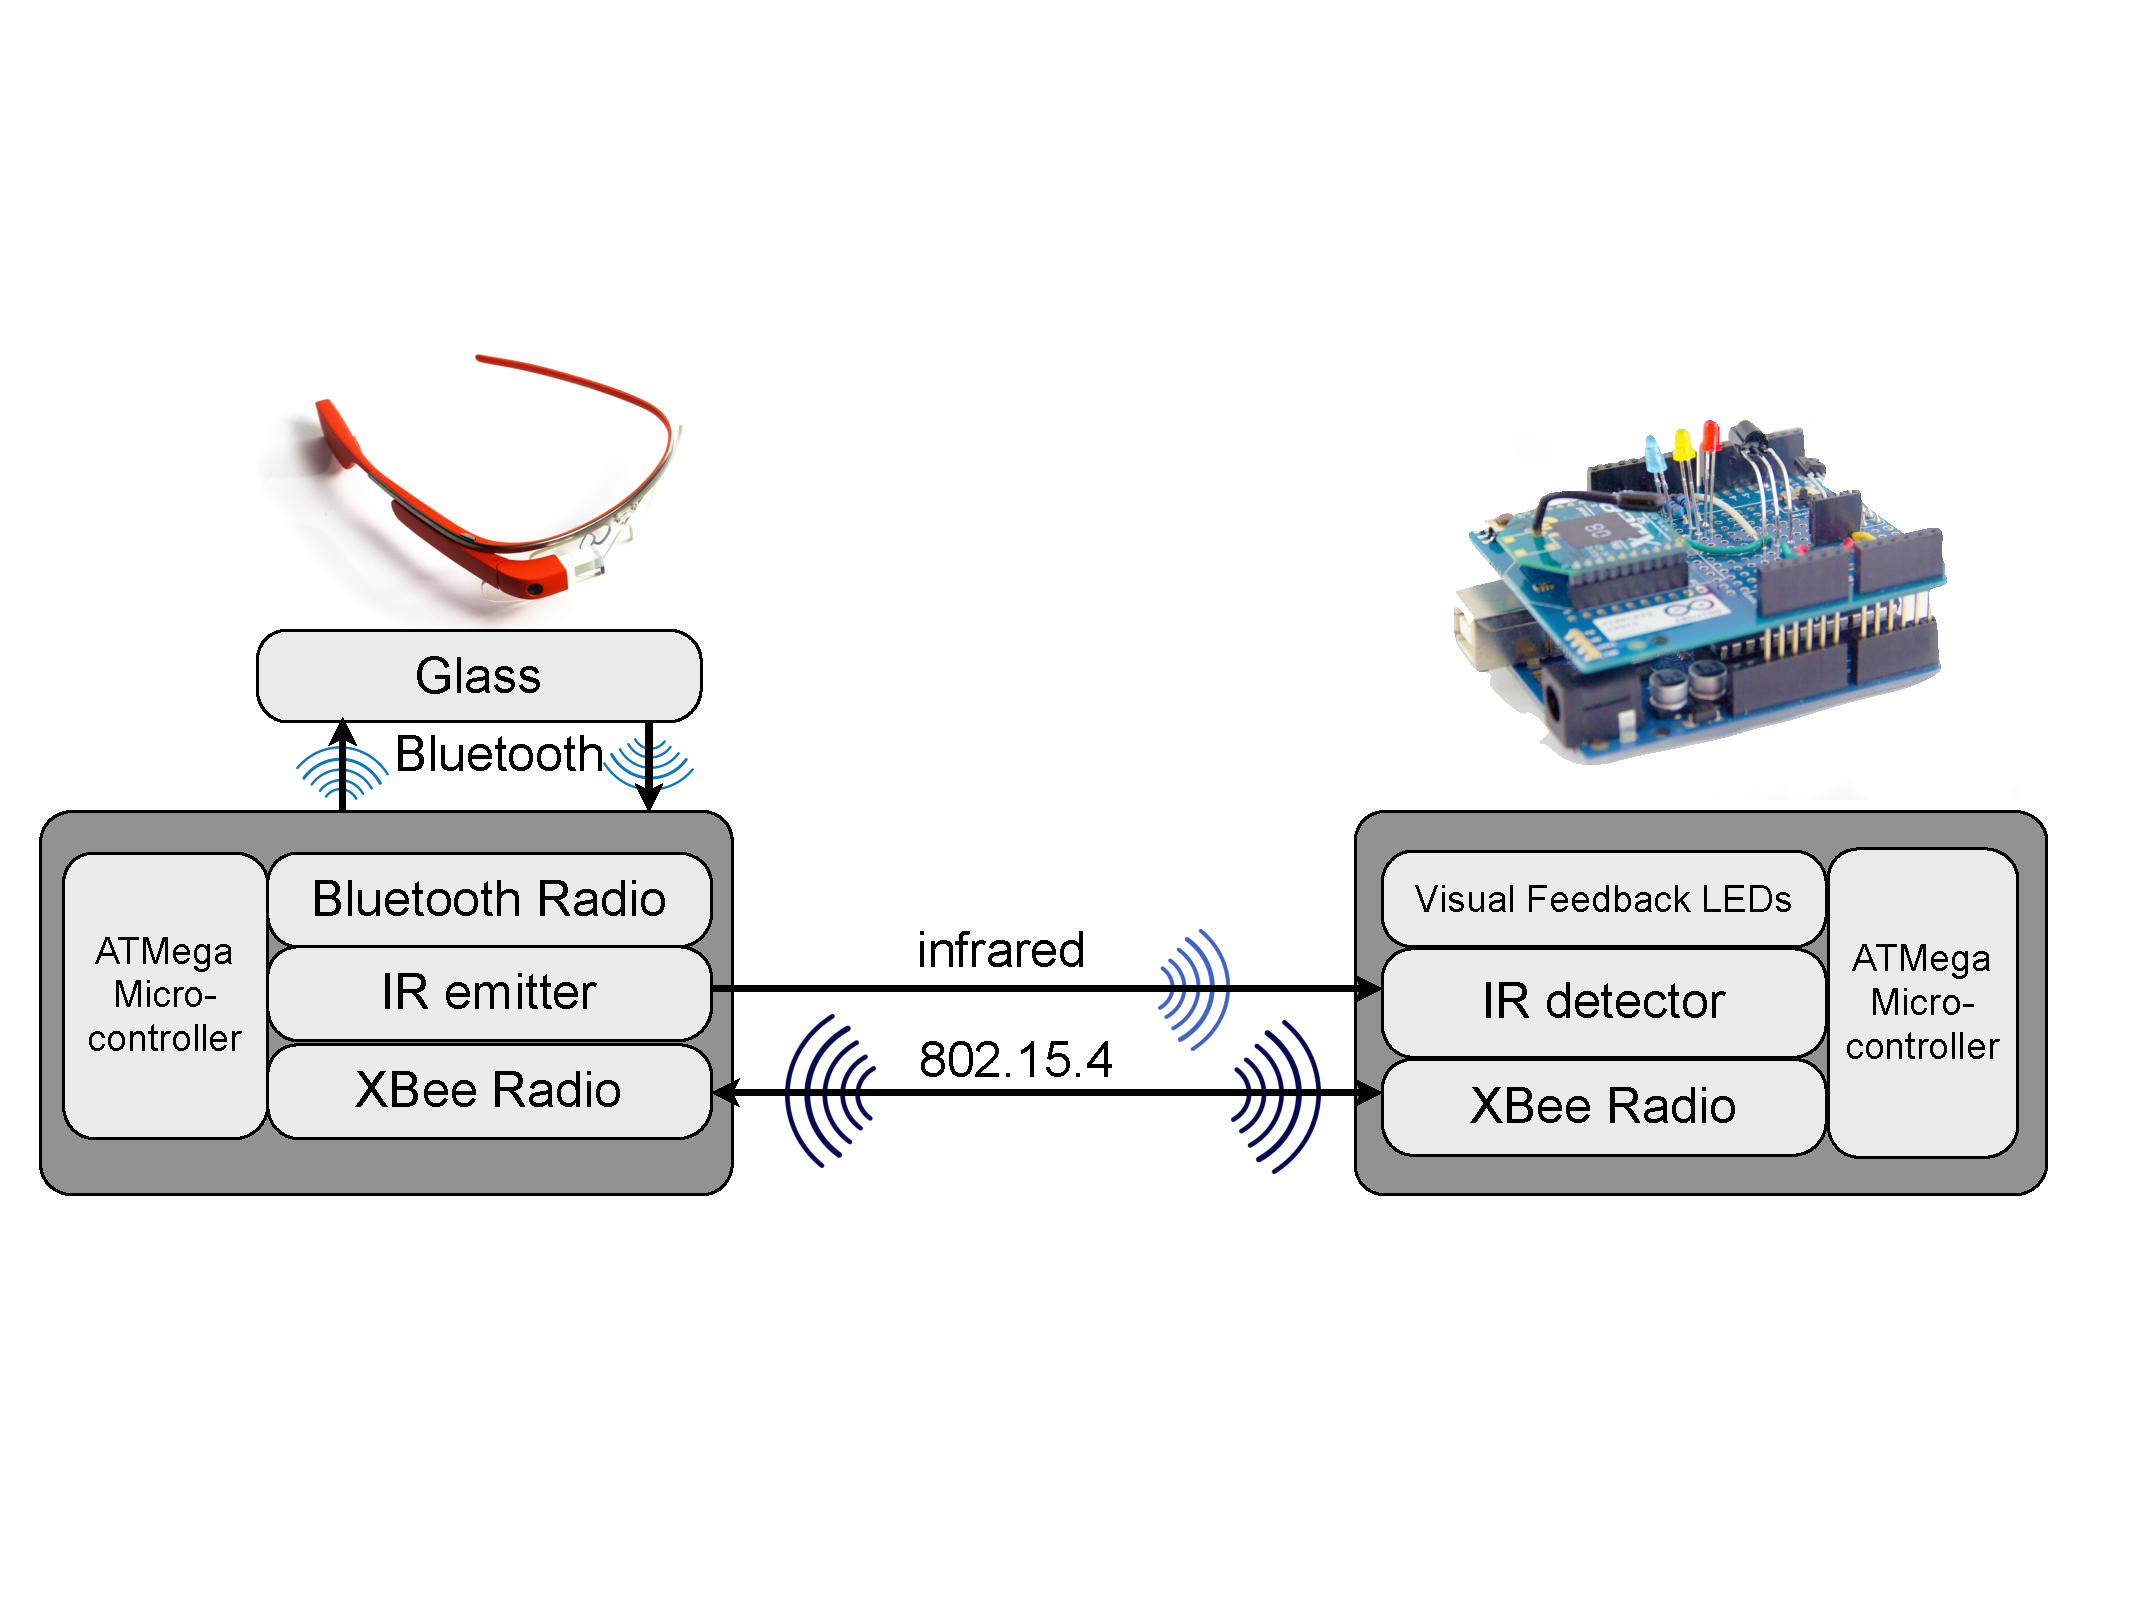
\includegraphics[width=0.95\columnwidth]{figures/architecture_new}
\caption{Our System architecture diagram. The selection is initiated through infrared but confirmed over 802.15.4.}
\label{fig:architecture}
\end{figure}

\newpage %bjoern hack fix
\subsection{Interaction Model}
From the user's perspective, interaction with \systemname proceeds in two stages (Figure~\ref{fig:interaction}): 


{\bf Scan:} The user first scans the environment to locate the position of the target. During this stage, Glass constantly sends out IR signals, and  targets offer immediate visual feedback when they receive a signal. The user confirms his desire to connect to a target by tapping on the Glass touchpad. Glass collects the responses from targets that have received IR reception through the backchannel of XBee. If there is only one single target in IR range, it is automatically selected. However, in a dense environment where multiple targets are within range, the user needs to refine his selection.


{\bf Refine:} When disambiguation is needed, the user must make an explicit selection among the targets within their view range. We have designed multiple refinement mechanisms -- all of which enable the user to select one from a subset of targets. The user confirms the current selection with a tap. Since the purpose of this stage is to disambiguate among potential targets, we will also use {\em disambiguation} to refer to this stage. Finally, a tap confirms a decision.


\begin{figure}[t!]
\centering
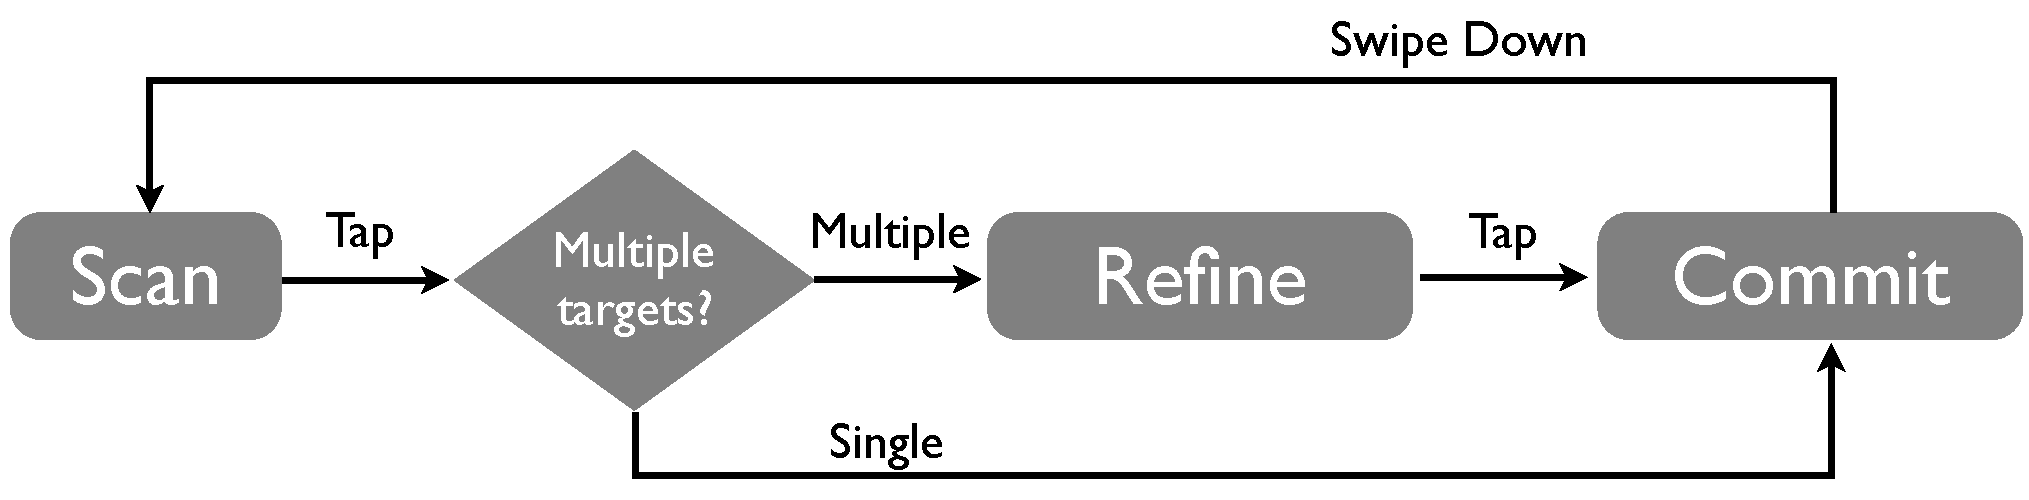
\includegraphics[width=\columnwidth]{figures/interactionModel2.pdf}
\caption{{\em scan} and {\em refine} -- two main stages during the interaction with HOBS. For completeness, we have also added the final state of {\em commit}.} 
\label{fig:interaction}
\end{figure}

The overall target acquisition time thus depends on scan and refine times, the probability that refinement is needed, and the time to commit an action (tap):
\begin{equation}
t_{total}=t_{scan}+P(refine)*t_{refine}+t_{commit}
\label{eq:time}
\end{equation}

In the following sections, we describe our iterative design and evaluation process to minimize the overall target selection time.

%%% Local Variables: 
%%% mode: latex
%%% TeX-master: "uist14"
%%% End: 

% \input{prototype}
% 
\section{Evaluation}
\label{sec:evaluation}

This section we present our work on the evaluation and user study.


%%% Local Variables: 
%%% mode: latex
%%% TeX-master: "uist14"
%%% End: 

% 
\section{Discussion}
\label{sec:discussion}

We discuss a few issues with the system.
%%% Local Variables: 
%%% mode: latex
%%% TeX-master: "uist14"
%%% End: 

% \section{Conclusion}
We introduced a novel method for selecting and controlling smart appliances in physical spaces through  infrared targeting based on head orientation. The design takes advantage of the fact that visual attention can express intention, makes it ituitive and helps users remain their focus in the physical world. It addresses the naming and scaling challenges faced by handheld mobile devices. While we present a prototype approach that requires that the user carry additional hardware, all parts can readily be miniaturized and integrated into future head-worn hardware. We also introduced a disambiguation technique in case head orientation is not sufficient to determine a unique target. We characterized our devices performance, arguing that it is matched well to the amount of head movement people can control without strain. A target acquisition study showed that the technique is efficient; a home control scenario showed promise but also limitations when trying to control complex appliances. As our environment continues to be populated by a swarm of sensing and actuation devices, methods to interrogate and control our smart environments may become increasingly important.
%\section{Acknowledgments}
%We thank our user study participants and the a

\iftoggle{anonymous}{
% no acks in anonymous submission
}{
  \section{Acknowledgments}
  
  This work was supported in part by the TerraSwarm Research Center, one of six centers supported by the STARnet phase of the Focus Center Research Program (FCRP) a Semiconductor Research Corporation program sponsored by MARCO and DARPA. Additional support was provided by a Sloan Foundation Fellowship and a Google Research Award.
}
%figure template:
%\begin{figure}[!h]
%\centering
%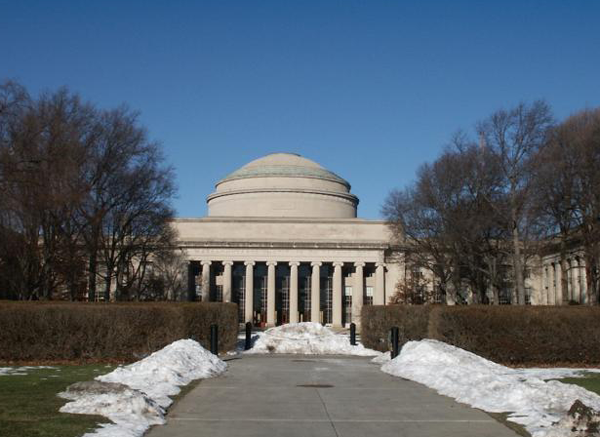
\includegraphics[width=1.0\columnwidth]{Figure1}
%\caption{With Caption Below, be sure to have a good resolution image
%  (see item D within the preparation instructions).}
%\label{fig:figure1}
%\end{figure}

% Balancing columns in a ref list is a bit of a pain because you
% either use a hack like flushend or balance, or manually insert
% a column break.  http://www.tex.ac.uk/cgi-bin/texfaq2html?label=balance
% multicols doesn't work because we're already in two-column mode,
% and flushend isn't awesome, so I choose balance.  See this
% for more info: http://cs.brown.edu/system/software/latex/doc/balance.pdf
%
% Note that in a perfect world balance wants to be in the first
% column of the last page.
%
% If balance doesn't work for you, you can remove that and
% hard-code a column break into the bbl file right before you
% submit:
%
% http://stackoverflow.com/questions/2149854/how-to-manually-equalize-columns-
% in-an-ieee-paper-if-using-bibtex
%
% Or, just remove \balance and give up on balancing the last page.
%
%% \balance

\bibliographystyle{acm-sigchi}
\bibliography{uist14}
\end{document}
